%!TEX root = ../xxxx-xx-xx_idamfro_masterthesis.tex
\chapter{The SMART project}
The SMART project was a \gls{cde} activity sponsored by the inspector general of the \gls{hv}, and executed by the \gls{ffi} in 2016. As stated in \cite{ep1667_bakgrunn} the purpose of the activity was to '...investigate whether commercial smart technology, primarily in the form of smart phones and/or tablets, can be used as a cheap and powerful platform for situational awareness for units that have little to no technological equipment available today.'. The goal of the SMART project was to investigate how \gls{cots} products can be used to enable information sharing with all the Armed Forces units, hence complement the current solution for information sharing. Figure \ref{fig:SMART_demo_sketch} show how the SMART solution can be connected with the current Information infrastructure and ensure information exchange with other units. The interface purposed between the server and INI in \cite{ep1667_bakgrunn} are with either using the current \gls{nffi} standard or by using service orientation as defined in \gls{fmn}. 

\begin{figure}
\label{fig:SMART_demo_sketch}
\centering
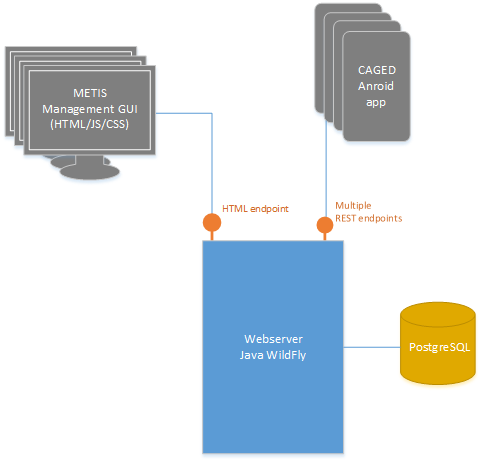
\includegraphics[width=0.8\columnwidth]{content/img/Titans_system_sketch.png}
\caption{The SMART demonstrator sketch \cite{ep1667_bakgrunn}}
\end{figure}

Through the project a demonstrator was developed and tested, and the results show that smart technology has great potential to complement the situational picture in military operations.
Through the next section the reader will get familiar with the organization and the intended user of the SMART project. Two main user groups with somewhat different requirements regarding information need, functionality and physical mobility will be identified. The second section of this chapter gives an overview of the developed prototype, its components and versions, while the last section provides an overview of the four tests that have been conducted by the SMART project. 

\section{The SMART user } \label{sec:smart_user}
The Norwegian Armed Forces are organized into five branches; the Army, the Navy, the Air Force, the \gls{hv} and the Cyber Defense. The \gls{hv} is the intended user of the SMART project and more precisely the area forces. \gls{hv} serves as a quick reaction force of the Armed Forces and their main responsibility is territorial protection. \gls{hv} consist of more than 45 000 soldiers distributed in four regions, 11 districts and 241 areas covering all over Norway\cite{forsvaret_home_guard}. The \gls{hv} is a mobilization force\footnote{Mobilization force means that the soldiers are not employed by the military on a daily basis, but train on a regular basis.} consisting of 15 \gls{isty} and 241 area forces. While the \gls{isty} are capable of rapid response and consists of highly trained and equipped personnel, the area forces have longer reaction time, are less equipped and the personnel have less training. The SMART project aims at providing a cheap communication system for the area forces, hence the user threshold has to be as small as possible, and the product has to be cheap and require as little management as possible.

\subsection{The command structure of HV}
As for any military unit, the command structure within \gls{hv} is very hierarchical see figure \ref{fig:hv_command_structure}. The smallest unit are squads which usually consists of about seven people, and are the soldiers on ground. Each squad member has a designated task and are lead by a squad leader. Squads usually operates as one unit, or at least within visual or auditory contact with their squad leader or their second in command. The squad leader executes the mission given by the platoon leader. A platoon is composed by three to five squads, which in turn are lead by the area command. Each level has one commander and one second in command. Higher up in the hierarchy there are additional roles like intelligence, operations, logistics, plans etc. 

Since the platoons are the soldiers on ground, they are highly mobile and has a rather limited information need compared to the area command staff. The area command staff, on the other hand, are usually located within a command post, are less mobile and need a broader situational picture. This leaves us with two main user groups - the \gls{hv} soldier and the staff members. The SMART project have developed two different interfaces, one for each of these user groups. The SMART Android App for situational awareness on squad and platoon level and a web interface for the staff members.


\begin{figure}
\label{fig:hv_command_structure}
\centering
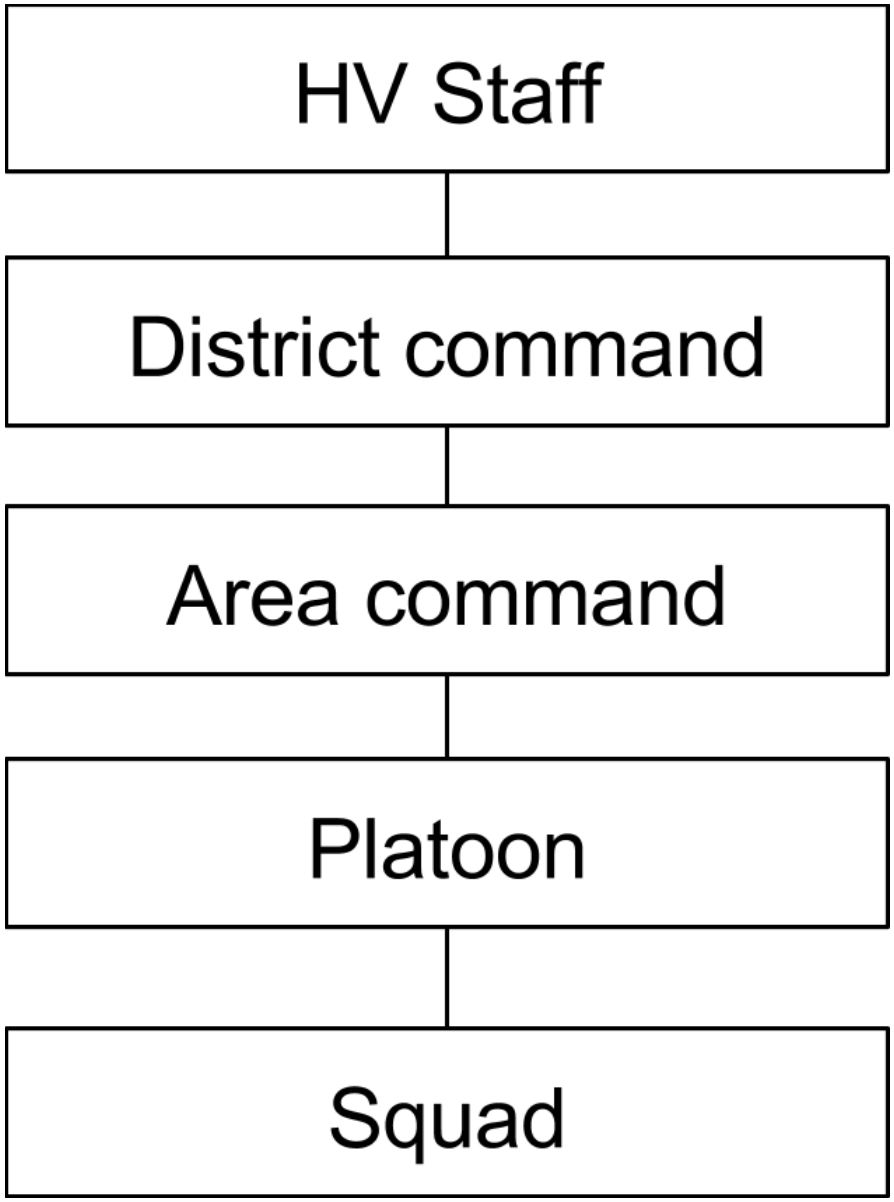
\includegraphics[width=0.4\columnwidth]{content/img/hv_command_structure.png}
\caption{\gls{hv} Command Structure}
\end{figure}

\subsubsection{The HV Soldier}
The \gls{hv} soldier is a person which have at least fulfilled one year of mandatory conscription some time in life and his/her age, background and experience can vary a lot \footnote{The age can vary from 18 - 55 years.\cite{lov_hv_2015}.} 
This accounts for both at the squad, platoon and area command level, however the commanders at each level and the people at the area command level usually have some additional training compared to the average soldier. 

\section{The TITANS and its components} \label{sec:titans_components}
The prototype developed through the SMART project is called the TITANS, and consists of three components - the smart phone App, a server component and a management interface, see figure \ref{fig:titans_architecture}.

\begin{figure}
\label{fig:titans_architecture}
\centering
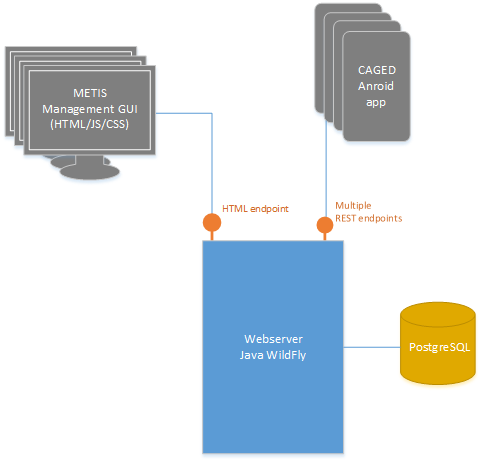
\includegraphics[width=0.8\columnwidth]{content/img/Titans_system_sketch.png}
\caption{TITANS architecture}
\end{figure}

\subsection{TITANS major versions}
Since the development of TITANS have followed an agile process the system have changed continuously. However, there are two major versions of the app to consider. The first version was developed as part of the bachelor thesis of three students from the Westerdals School of Arts, Communication and Technology during spring 2016. Their bachelor thesis \cite{gudmundsen_communication_2016} gives insight into the process of designing and developing the basic functionality for the \gls{caged} app and the server component, as well as an overview of the findings when testing it during week 17. Based on the results from this test the system was enhanced by some summer students, which implemented some major changes like adding groups, enhancing location tracking, and added the management interface called METIS. 

\subsection{TITANS security}
VPN
NFC user authentication

\section{The SMART project tests}
Table \ref{tab:smart_tests} gives an overview of the four tests that has been conducted by the SMART project. 
\begin{table}[]
\centering
\caption{The SMART project User tests}
\label{tab:smart_tests}
\begin{tabular}{|l|l|l|l|l|l|l|}
\hline
W & Location   & Duration      & Users & Ver & Activity & Comment       \\ \hline
17        & Domb{\aa}s     &  5 days              & 50  & 1  & Course & 24 h cycle \\ \hline
33        & Domb{\aa}s     &   5 days            & 42   & 2 & Course &               \\ \hline
36        & Tr{\o}ndelag  &  40 hours              & 16  & 2 & Exercise &    Used by red team\footnotemark           \\ \hline
39        & Hauerseter  & $\sim$40 hours & 33   & 2  & Exercise         &               \\ \hline
\end{tabular}
\end{table}
\footnotetext{Red team are used in exercises to train the personnel, and are playing the opponent of the blue team, the training personnel. To ensure maximum effect the red team usually gets more information (like the blue team mission and their likely movement), and the missions are usually of shorter duration.}

For all four tests, the following facts accounts:
\begin{itemize}
	\item{No user have participated on more than one test}
	\item{There have not been given any instruction on how to use the app, except a small how-to folder with the size of a credit card}
	\item{The system have been used as a tool for the soldiers to solve their main mission\footnote{This have given a valuable insight of the usability of the system.}. }
	\item{The devices have been from at least three different vendors}
	\item{\gls{ffi} have preconfigured the server and the user credentials}
\end{itemize}

From table \ref{tab:smart_tests} it is important to notice that version one was used during the first test, hence it should be given less weight when analyzing the results. It is also important to notice that the user group and the context have varied slightly form each test. During the first and second test the system was used by \gls{hv} soldiers participating at a commanders course, hence their motivation, experience and level of training can be expected to be a bit higher compared to the average user. During the third test the system was used by the red team, which differ slightly from the intended usage, however the results are still applicable. The last test is the test which is most similar to the intended usage and best represent the user group and this test should be given most weight.  

\begin{figure}
\label{fig:user_test_timeline}
\centering
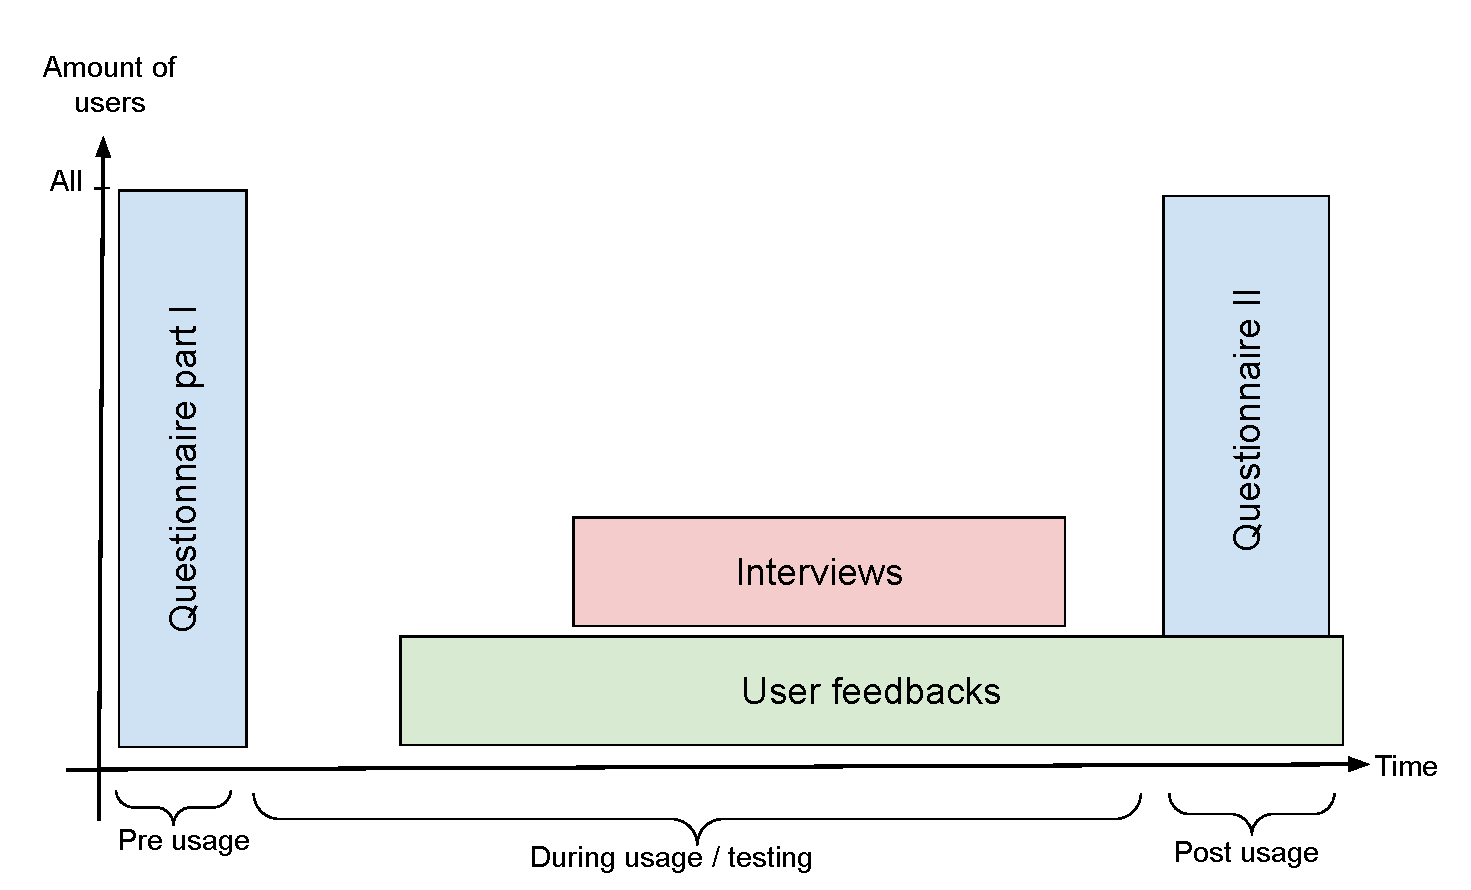
\includegraphics[width=1\columnwidth]{content/img/tests_timeline.pdf}
\caption{User test execution}
\end{figure}
Before, during and after each test a large amount of data was gathered. Figure \ref{fig:user_test_timeline} visualize the method used to gather user feedback and at what time in the test cycle it happened. As the figure shows, the methods used are questionnaires, interviews and informal conversation with the user. 



\subsection{Questionnaires}
Before and after each test, the users were asked to answer a questionnaire, referred to as questionnaire part I and part II. The questionnaires were written by some statistics experts at \gls{ffi} and included both closed-ended matrix questions and open-ended questions. The intent of the part I questionnaire was to uncover the users experience, habit and attitude of using smart technology, as well as their expectation to the developed app. The part II questionnaire gathered data about the experience from the actual usage and what potential the user saw in smart technology. 

\subsection{Interviews}
Interviews were only conducted during week 17 and 39. For the first test, a focus group of five persons were selected to represent different types of users and attitude to the system. The interviews were preformed during the execution of the test. For test two and three no formal interviews were conducted, while for the last test the user of Metis were interviewed, to gain insight into the administrator platform. 

\subsection{Other user feedback}
During the execution of the tests, a support chat room were configured enabling the users to communicate directly with the \gls{ffi}. The conversation logs both gives insight into what the user had difficulties with as well as some new requirements and proposal for enhancements were posted. In addition to the chat room \gls{ffi} met the users in different occasions both during and after the execution and in field and at the operation center. 
